\documentclass[class=myArticleClass, float=false, crop=false]{standalone}

%=====================================================================
% Introduction
%=====================================================================
\begin{document}

\section{Introduction}
This is an introduction. Testing one, two, three.

Acronyms: \ab{re}

Glossary: \gls{limitation}

Reference: \cite{knuthwebsite}

\begin{figure}[h]
	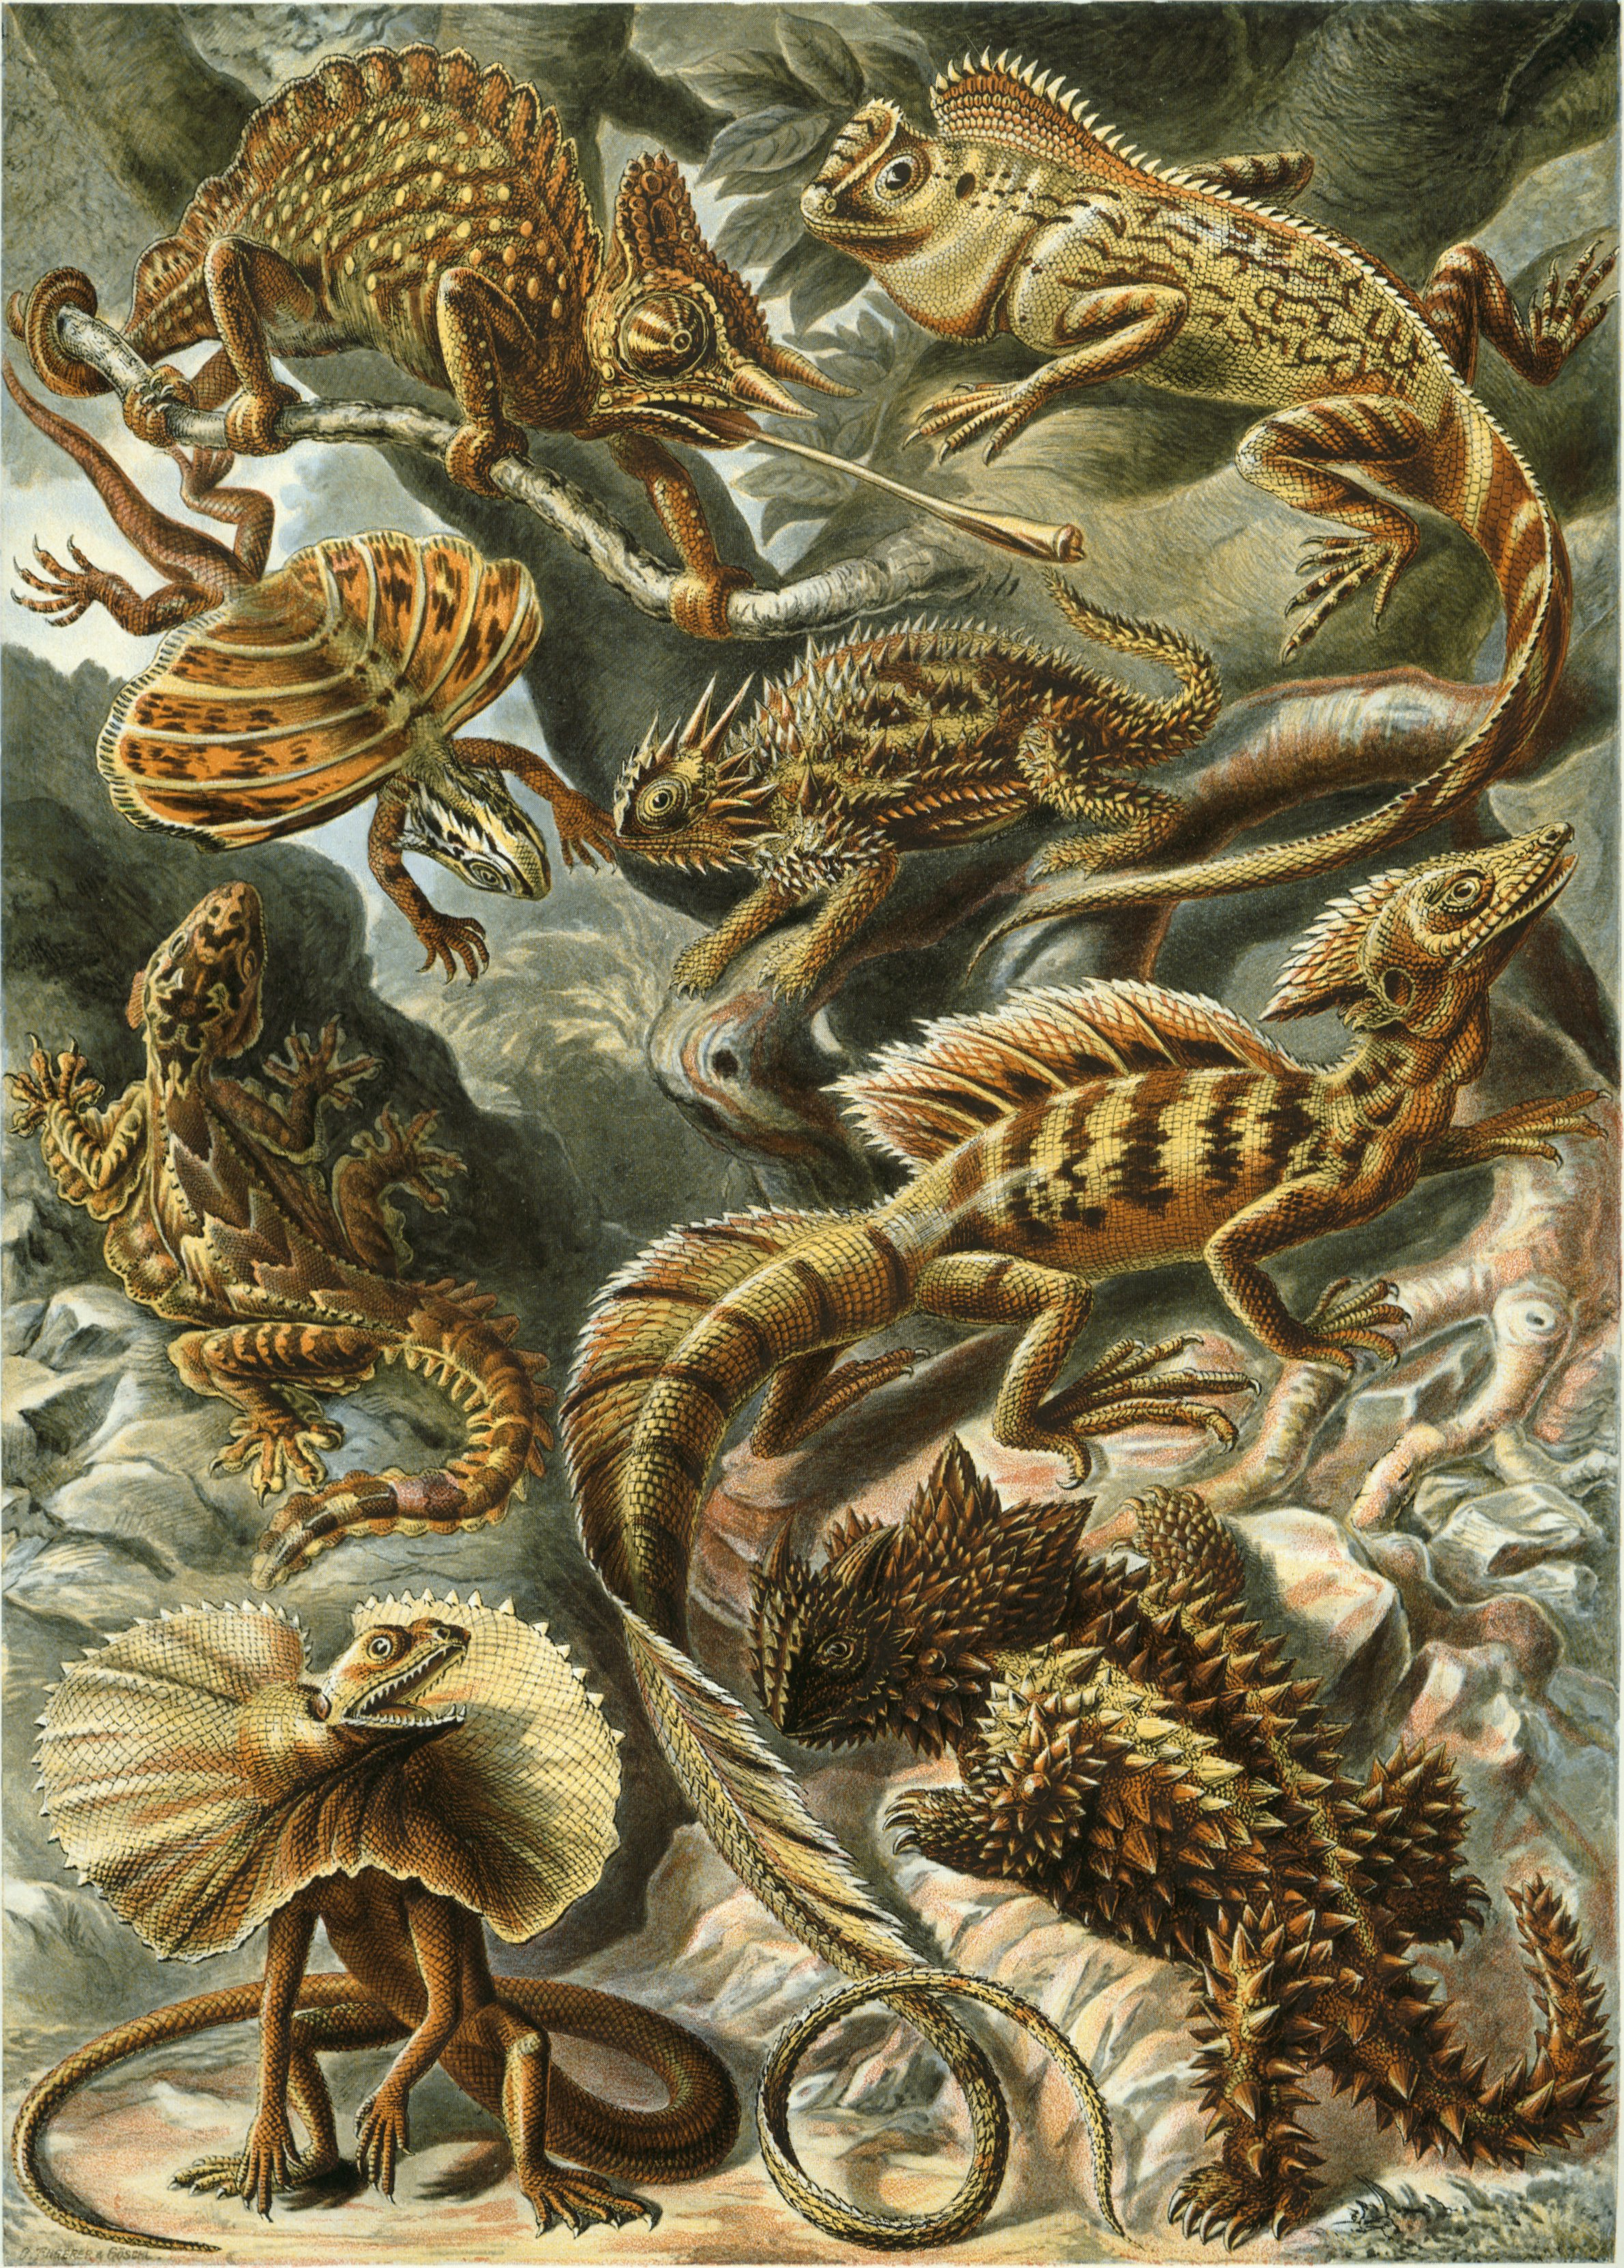
\includegraphics[scale=0.1]{ImageTest}
	\label{fig:mesh1}
	\caption{Kunstformen der Natur (1904), plate 79: Lacertilia}
\end{figure}

\begin{table}[h!]
	\centering
	\begin{tabular}{||c c c c||} 
	 \hline
	 Col1 & Col2 & Col2 & Col3 \\ [0.5ex] 
	 \hline\hline
	 1 & 6 & 87837 & 787 \\ 
	 2 & 7 & 78 & 5415 \\
	 3 & 545 & 778 & 7507 \\
	 4 & 545 & 18744 & 7560 \\
	 5 & 88 & 788 & 6344 \\ [1ex] 
	 \hline
	\end{tabular}
	\caption{Table to test captions and labels.}
	\label{tab:1}
\end{table}

\end{document}